\documentclass{article}
\usepackage[utf8]{inputenc}
\usepackage[T1]{fontenc}
\usepackage{graphicx}
\usepackage[a4paper]{geometry}
\usepackage{helvet}
\usepackage[pdftex]{hyperref}
\usepackage{pdfpages}
\usepackage{lscape}
\usepackage{changepage}
\usepackage{xcolor}
\usepackage{fancyhdr}
\usepackage{lastpage}


\hypersetup{
	pdfauthor={Bruno Lorenz},
	pdftitle={ExporterBundle Documentation},
	colorlinks=true,
  linkcolor=blue
}

%###############################################################################################
\title{ExporterBundle Documentation}
\author{Bruno Lorenz\\
  Namics AG\\
  Watzmannstraße 1a\\
  81541 München\\
  Germany\\
  \texttt{bruno.lorenz@namics.com}}
\date{\today}

%###############################################################################################
\definecolor{wmark1}{HTML}{9B1329}
\definecolor{wmark2}{HTML}{FF0000}
\definecolor{wmark3}{HTML}{009036}
%###############################################################################################

\pagestyle{fancy}

\fancyhead{}
\cfoot{}

\renewcommand{\headrulewidth}{0pt}


\renewcommand{\familydefault}{\sfdefault}
\renewcommand{\baselinestretch}{1.10}\normalsize

\def\Version#1{\def\version{#1}}
\Version{0.1a}
%###############################################################################################
\newcommand{\litem}[1]{
	\vspace{-0.2cm}
	\item{#1}
}

\newcommand{\hsection}[1]{
  \hypertarget{chap-#1}{\section{#1}}
}

\newcommand{\hsubsection}[1]{
 \hypertarget{sec-#1}{\section{#1}}
}

%###############################################################################################


\begin{document}

\begin{titlepage}
\begin{center}
  \begin{minipage}{\textwidth}
    \fontsize{18}{22}
    \selectfont
    \raggedright
    \textcolor{wmark1}{Ambition. Begeisterung.} \textcolor{wmark2}{Herzblut.} \textcolor{wmark1}{Felxibilität. Netzwerk. Technik aus Leidenschaft.} \textcolor{wmark3}{München.}
  \end{minipage}

  \begin{minipage}{0.8\textwidth}
    \vspace{3.5cm}
    \Huge ExporterBundle \\[0.4cm]
    \LARGE Documentation v\version\\
    \\
    \normalsize \today
  \end{minipage}

  \begin{minipage}{\textwidth}

  \end{minipage}
\end{center}
\end{titlepage} \newpage

\noindent \textbf{\Large Versionhistory}\\

\newcommand{\versionrow}[4]{
    \hdashline
    \small #1 &
    \small #2 &
    \small #3 &
    \small #4 \\
}


\begin{table}[h]
    \begin{tabular*}{\textwidth}{l:l:l:l}
        \hline
        \versionrow{\textbf{Version}}{\textbf{Date}}{\textbf{Author}}{\textbf{Description of changes}}
        \hline
        \versionrow{v0.1a}{2012-01-04}{Bruno Lorenz}{Initial document}
        \versionrow{v0.2a}{2012-01-05}{Bruno Lorenz}{Updated composer configuration settings}
        \hline
    \end{tabular*}
\end{table}

 \newpage


\lfoot{ExporterBundle Documentation}
\rfoot{\textnormal{\thepage} / \textnormal{\pageref*{LastPage}}}
\renewcommand{\footrulewidth}{0.4pt}
\setcounter{page}{1}
\tableofcontents \newpage



\section{Installation}


% ################################################################################################################################
\subsection{Requirements}
During some functionality is only available since symfony 2.1 it is \textbf{necessary to have your project on a symfony 2.1 basis}. Some actions requires additional tools to do their work. \textbf{As long as this actions are part of the actionstack they will force you to have this tools installed and callable!} If you don't need this action and don't want to install the tools needed for it you have to configure a action stack without this specific action. See chapter '\mbox{\hyperlink{chap-Configuration}{Configuration}}' for more information about defining you own action stack.

% ################################################################################################################################
\subsection{Dependency management}
Update your composer.json and add a new repository. \\

\begin{verbatim}
{
"type" : "vcs",
"url"  : "http://github.com/senuphtyz/TerrificExporterBundle"
}
\end{verbatim}

\noindent After that add a new requirement to your project. \\

\begin{verbatim}
"senuphtyz/terrific-exporter-bundle" : "v2.*"
\end{verbatim}
\noindent Now update your project using the composer. \\

\begin{verbatim}
php composer.phar update
\end{verbatim}
\noindent This should now install alle necessary requirements for your project. \\

% ################################################################################################################################
\subsection{Tooling}
There are a number of tools needed depending on your configuration and tasks.\\

\begin{itemize}
	\litem{YUIDoc}
	\litem{csshint}
	\litem{jslint}
	\litem{jpegoptim}
	\litem{optipng}
	\litem{advpng}
	\litem{montage}
    \litem{diff}
\end{itemize}

\noindent It is necessary to have all tools within path, the exporter won't search for tools on your hardrive. So you have to setup your path variable depending on your os system correctly to have all tools within path's.\\
\\
On Windows: \url{http://www.computerhope.com/issues/ch000549.htm}\\
\\
On *nix/MacOSX: \url{http://www.troubleshooters.com/linux/prepostpath.htm}\\
To do a permanent change it is necessary to change ~/.bashrc or ~/.bash\_profile depending on your os.

% ################################################################################################################################
\subsubsection{YUIDoc, jslint, csshint}
YUIDoc, jslint and csshint are installed using Node.js. Just go to nodejs.org download the package fits for you operating system and install it. \\
After the installation is done open up a new commandline and install Node.js.

\begin{verbatim}
npm -g install yuidocjs jslint csshint
\end{verbatim}

\noindent For further help and syntax for YUIDoc visit \url{http://yui.github.com/yuidoc/}.


% ################################################################################################################################
\subsubsection{jpegoptim, optipng, advpng, montage}

% ################################################################################################################################
\noindent \textbf{Windows}\\
\noindent Jpegoptim is currently not available on Windows systems.\\
\\
Optipng can be retrieved from \mbox{\url{http://optipng.sourceforge.net/}}. Just download the Windows package unzip it no installation required.\\
\\
Advpng or advancecomp can be fetched from \mbox{\url{http://advancemame.sourceforge.net/comp-download.html}}. The same just download and unzip.\\
\\
Montage is part of the ImageMagick toolset. To install ImageMagick visit:\\
\mbox{\url{http://www.imagemagick.org/script/binary-releases.php}} \\

% ################################################################################################################################

\noindent \textbf{Unix/Linux}\\
\noindent On Ubuntu/Debian based Linux it is possible to install jpegoptim directly using your package manager.\\


\begin{verbatim}
sudo apt-get install jpegoptim advancecomp optipng imagemagick
\end{verbatim}

\noindent
On RHEL/Fedora/Centos Linux you have to install jpegoptim from source, rest of the tools could be installed using yum. Download the current version from \url{http://www.kokkonen.net/tjko/projects.html}. \\


\begin{verbatim}
sudo yum install advancecomp optipng ImageMagick
\end{verbatim}

\noindent \textbf{jpegoptim}
\begin{verbatim}
tar zxf jpegoptim-1.2.4.tar.gz
cd jpegoptim-1.2.4
./configure && make && make install
\end{verbatim}


% ################################################################################################################################
\noindent \textbf{MacOSX}\\
\noindent On MacOSX the easiest way to get the whole toolset is to install ImageOptim. This application contains all necessary image optimizing tools needed by the exporter.\\
\\
\url{http://imageoptim.com/}\\
\\
Montage is part of the ImageMagick toolset. To install ImageMagick visit:\\
\url{http://www.imagemagick.org/script/binary-releases.php}\\


% ################################################################################################################################
\subsubsection{diff}

\noindent \textbf{Windows}\\
\noindent On windows there are a number of tools doing the same job as diff on *nixes. You can install a commandline version from diff with \mbox{\href{http://www.cygwin.com/}{cygwin}}.

\noindent \textbf{Unix/Linux}\\
\noindent Normally diff should be installed on all *nixes. If not just install it using your packagemanager. \\
\begin{verbatim}
# Debian/Ubuntu:
sudo apt-get install diff

# RHEL/CentOS/Fedora:
sudo yum install diff
\end{verbatim}

\noindent \textbf{MacOSX}\\
\noindent On MacOSX diff is already installed.



% ################################################################################################################################
\subsection{Setup an export environment}

It is necessary to setup a new environment for you export. To setup an export environment just copy your app/config.yml to app/config\_export.yml. Now you created a new environment called "export". \\
\\
You can now configure the environment to your project needs. For further information visit \url{http://symfony.com/doc/current/cookbook/configuration/environments.html}.\\

\section{Configuration}

All configuration goes beyond a terrific\_exporter node within the config\_export.yml.\\
\\
\textbf{build\_local\_paths: (true/false)}\\
If build\_local\_paths is enabled the exporter will change all urls within html and css files to \\match within the exported package.\\
\\
\textbf{build\_js\_doc: (true/false)} \\
Enables the export of a javascript documentation. The documentation is generated using YUIDoc. \\
\\
\textbf{build\_settings: (path)}\\
This setting should target to a build.ini file. Within this file there are only settings for the \\projektname an versioning data.\\
\\
\textbf{build\_path: (path)}\\
Has to target to a path which is the export target path.\\
\\
\textbf{export\_with\_version: (true/false)}\\
Set to true if the exporter should build zips/folders with version numbers within its name.\\
\\
\textbf{autoincrement\_build: (true/false)}\\
True if the exporter should increase the revision after each build.\\
\\
\textbf{validate\_js: (true/false)}\\
Activates the validation of javascript. Validation is done using jshint.\\
\\
\textbf{validate\_css: (true/false)}\\
Activate the validation of css. Validation is done using csshint.\\
\\
\textbf{optimize\_image: (true/false)}\\
Set to true to optimize images in the output directory. Optimization is done using jpegoptim, \\optipng and advpng.\\
\\
\textbf{export\_views: (true/false)}\\
Activates the export of the views marked with a @Export annotation.\\
\\
\textbf{export\_modules: (true/false)}\\
Activates the export of plain module html. The url within this modules are not rewriten even if \\the build\_local\_paths option is activated.\\
\\
\textbf{export\_type: (string: folder/zip)}\\
Set the export type if the export should be done as folder or as a zip.\\
\\
\textbf{build\_actions: (list of objects)}\\
These option allows to setup a build chain. Here you can append project related exporting tasks or change the buildin order.\\
\\
\textbf{sprites: (list of objects)}\\
Here you can setup sprite information. The exporter will build the sprites with the given data.\\
\\


\subsection{Example configuration}

\begin{verbatim}

terrific_exporter:
	build_local_paths:        true
	build_js_doc:             true
	build_settings:           "build/build.ini"
	build_path:               "build/"
	export_with_version:      false
	autoincrement_build:      true
	validate_js:              false
	validate_css:             false
	validate_html:            false
	optimize_images:          true
	export_views:             true
	export_modules:           true
	export_type:              folder

	build_actions:
	      - Terrific\ExporterBundle\Actions\ClearAction
	      - Terrific\ExporterBundle\Actions\BuildJSDoc
	      - Terrific\ExporterBundle\Actions\ValidateJS
	      - Terrific\ExporterBundle\Actions\ValidateCSS
	      - Terrific\ExporterBundle\Actions\ValidateModules
	      - Terrific\ExporterBundle\Actions\ValidateViews
	      - Terrific\ExporterBundle\Actions\GenerateSprites
	      - Terrific\ExporterBundle\Actions\ExportImages
	      - Terrific\ExporterBundle\Actions\ExportAssets
	      - Terrific\ExporterBundle\Actions\OptimizeImages
	      - Terrific\ExporterBundle\Actions\ExportModules
	      - Terrific\ExporterBundle\Actions\ExportViews

	sprites:
	      - { directory: "PROD/internet_sprite_icons", target: "web/img/sprite_icons.png", item: { height: 50, width: 100 }}

\end{verbatim}
\newcommand{\cmdoptiondesc}[2]{
    \noindent \textbf{#1}\\
    \vspace{-1em}
    \begin{adjustwidth}{\parindent}{0cm}
        #2
    \end{adjustwidth}
    \vspace{1em}
}


\hsection{Usage}

To startup an export use the following command.

\begin{verbatim}
    app/console build:export --env=export --no-debug
\end{verbatim}



\subsection{Commandline options}

\cmdoptiondesc{--no-image-optimization}{
    Overrides configuration setting optimize\_images and starts the chain without optimizing Images. Skip actions:
    \begin{itemize}
          \item{Terrific\textnormal{\textbackslash}ExporterBundle\textnormal{\textbackslash}Actions\textnormal{\textbackslash}OptimizeImages}
    \end{itemize}
}

\cmdoptiondesc{--no-js-doc} {
    Do not build a javascript documentation for this export run. This does skip the following actions:
    \begin{itemize}
        \item{Terrific\textnormal{\textbackslash}ExporterBundle\textnormal{\textbackslash}Actions\textnormal{\textbackslash}BuildJSDoc}
    \end{itemize}
}

\cmdoptiondesc{--no-validation} {
    Ignores validation configuration and skip the following actions:
    \begin{itemize}
          \item{Terrific\textnormal{\textbackslash}ExporterBundle\textnormal{\textbackslash}Actions\textnormal{\textbackslash}ValidateJS}
          \item{Terrific\textnormal{\textbackslash}ExporterBundle\textnormal{\textbackslash}Actions\textnormal{\textbackslash}ValidateCSS}
          \item{Terrific\textnormal{\textbackslash}ExporterBundle\textnormal{\textbackslash}Actions\textnormal{\textbackslash}ValidateModules}
          \item{Terrific\textnormal{\textbackslash}ExporterBundle\textnormal{\textbackslash}Actions\textnormal{\textbackslash}ValidateViews}
    \end{itemize}
}


\subsection{Annotations}

\noindent
\begin{minipage}{\textwidth}
\textbf{@Export}\\
\vspace{-1em}
\begin{adjustwidth}{\parindent}{0cm}
To export a view it is necessary to annotate a controller method with this annotation. It is possible to control a set of options for each view directly within this annotation. This example is only valid if you don't have to export a localized version of a view. If no environment is given this view will exported in all environments.

\begin{verbatim}
 @Export(
     name="viewname.html",
     environment="env1,env2,..."
 )
\end{verbatim}
\end{adjustwidth}
\vspace{1em}
\end{minipage}

\noindent
\begin{minipage}{\textwidth}
\textbf{@LocaleExport}\\
\vspace{-1em}
\begin{adjustwidth}{\parindent}{0cm}
Each view must have their own for each locale which should exported. To set different settings for each locale you have to use the @LocaleExport annotation. This annotation is used in combination with the @Export annotation. Setting up locale exportation will disable exporting the default language which means you have to annotate \textbf{all} locales that should exported. If no environment is given this view will exported in all environments. \\
\\
Usage with @Export:
\begin{verbatim}
@Export(
    @LocaleExport(name="viewname_de.html", locale="de"),
    @LocaleExport(name="viewname_en.html", locale="en", environment="env1"),
    @LocaleExport(name="viewname_lv.html", locale="lv", environment="env2"),
    ....
)
\end{verbatim}
\end{adjustwidth}
\vspace{1em}
\end{minipage}


\hsection{Debugging}

\subsection{Configuration}

\begin{verbatim}
services:
    terrific.formatter.line:
        class: Monolog\Formatter\LineFormatter
        arguments:
            - "[%%datetime%%] [%%level_name%%]: %%message%%\n"

monolog:
    handlers:
        file:
            type:  stream
            path:  %kernel.logs_dir%/%kernel.environment%.log
            level: debug
            formatter: terrific.formatter.line
\end{verbatim}

\noindent
Add this snippet to your export environment configuration.
This snippet will activate logging to a file called like your environment beyond the app/logs directory. The loglevel debug will output a massive amount of logging from the exporter. Currently only the log file contains a list of validation errors for your css / js files. For more information about how to configure your monolog see \url{http://symfony.com/doc/current/cookbook/logging/monolog.html}.
\hsection{Actions}

All buildin actions are documented within these chapter. This maybe have some helpful information when you have to build your own action chain.

\noindent \begin{minipage}{\textwidth}
\vspace{1.5em}
\hypertarget{sec-Actions-ClearAction}{\subsection{Terrific\textnormal{\textbackslash}ExporterBundle\textnormal{\textbackslash}Actions\textnormal{\textbackslash}ClearAction}}

This action simple just clear all data from the target directory. If configuration option 'export\_with\_version' is activated this action does simply nothing cause normally the export folder should not exists during startup.
\end{minipage}

\noindent \begin{minipage}{\textwidth}
\vspace{1.5em}
\hypertarget{sec-Actions-BuildJSDoc}{\subsection{Terrific\textnormal{\textbackslash}ExporterBundle\textnormal{\textbackslash}Actions\textnormal{\textbackslash}BuildJSDoc}}
BuildJSDoc will first test if yuidoc is callable. After that test it look for a suitable yuidoc.json file, if a file has been found the action starts the yuidoc command with the found configuration. \\
\\
An example call could look like this, and is going to be called withing the current project folder.
\begin{verbatim}
yuidoc -c /data/symfony2-project/app/config/yuidoc.json
\end{verbatim}
\end{minipage}

\noindent \begin{minipage}{\textwidth}
\vspace{1.5em}
\hypertarget{sec-Actions-ValidateJS}{\subsection{Terrific\textnormal{\textbackslash}ExporterBundle\textnormal{\textbackslash}Actions\textnormal{\textbackslash}ValidateJS}}
Javascript will be validated within this action. This action will get a list of all necessary javascript assets from the PageManager class. After retrieving this list it temporary removes the min filters and place the content for \textbf{each part} of the asset within a temporary file. After saving that file the jslint command will looking for a suitable configuration file an starts to verify the contents of the temp file. \\
\\
An example call could look like this:
\begin{verbatim}
jshint --jslint-reporter --config /sf2-prj/app/config/jshint.json /tmp/ZIEASDZER
\end{verbatim}
\end{minipage}


\noindent \begin{minipage}{\textwidth}
\vspace{1.5em}
\hypertarget{sec-Actions-ValidateCSS}{\subsection{Terrific\textnormal{\textbackslash}ExporterBundle\textnormal{\textbackslash}Actions\textnormal{\textbackslash}ValidateCSS}}
Stylesheets will be validated using this actions. This action also retrieves a list of all potential used style assets from the PageManager class. After retrieving this list the minfilter will be removed for dumping the content \textbf{each part} the asset to a temp files.\\
\\
Example for the csslint validation command:
\begin{verbatim}
csslint
    --format=lint-xml
    --errors=[from cfg]
    --warning=[from cfg]
    --ignore=[from cfg]
    /tmpdir/ASDFETZ
\end{verbatim}
\end{minipage}

\noindent \begin{minipage}{\textwidth}
\vspace{1.5em}
\hypertarget{sec-Actions-ValidateModules}{\subsection{Terrific\textnormal{\textbackslash}ExporterBundle\textnormal{\textbackslash}Actions\textnormal{\textbackslash}ValidateModules}}
First of all this action has a additional requirement on the configuration. This configuration must have enabled the options 'validate\_html' and 'export\_modules'. If one of them is not activated this action will be skipped. After starting this action it retrieves a list of all module combinations (module <-> skin <-> view) from the PageManager class. The modules are exported without any HTML from the view, just the plain modules. After exporting this HTML to a temp file the action try's to send this file to the W3CValidator (\url{http://validator.w3.org/}). Its required to have a internet connection to start this action. \\
\\
To generate a valid HTML ValidateModule uses a template file. This template file (module-template.tpl.html) can be replaced by placing a file with the same name in your app/config folder. Within this file just two variables are special \mbox{'\%MODULE\_NAME\%'} and \mbox{'\%MODULE\_CONTENT\%'}. Both variables are replaced with the corresponding content before sending to the W3CValidator.
\end{minipage}

\noindent \begin{minipage}{\textwidth}
\vspace{1.5em}
\hypertarget{sec-Actions-ValidateViews}{\subsection{Terrific\textnormal{\textbackslash}ExporterBundle\textnormal{\textbackslash}Actions\textnormal{\textbackslash}ValidateViews}}
This action handles the validation for the views just like the ValidateModules action. The difference between this both action are that ValidateViews requires other configuration options to start ('export\_views' and 'validate\_html'). The views also have all source code from the used modules within this view. This ValdationAction also uses the W3CValidator.
\end{minipage}

\noindent \begin{minipage}{\textwidth}
\vspace{1.5em}
\hypertarget{sec-Actions-GenerateSprites}{\subsection{Terrific\textnormal{\textbackslash}ExporterBundle\textnormal{\textbackslash}Actions\textnormal{\textbackslash}GenerateSprites}}
GenerateSprites needs some more configuration than the other actions. Each sprite which should be generated must have an entry within the config file. If there is no configured sprite(s) the action will just be skipped. To generate a sprite this action uses the montage tool from the ImageMagick toolset. After retrieving a filelist for merging as a sprite the action will sort this files by name. This offers you the possibility to order you images within your sprite. Filenames like 0000\_arrow.png are best practice. If this file is part of the export, which should be the normal usecase, this action has to \textbf{run before ExportImages}.\\
\\
Example for a sprite generation call:
\begin{verbatim}
montage
    -mode Concatenate
    -tile x${height * count images}
    -geometry ${width}x${height}+0+0
    -bordercolor none
    -background none
    ${list of files} ${target}
\end{verbatim}
\end{minipage}

\noindent \begin{minipage}{\textwidth}
\vspace{1.5em}
\hypertarget{sec-Actions-ExportImages}{\subsection{Terrific\textnormal{\textbackslash}ExporterBundle\textnormal{\textbackslash}Actions\textnormal{\textbackslash}ExportImages}}
All images which are used within the exported views should be exported by ExportImages. To control which image is part of the export you have to encapsulate each image within the \textbf{Twig's asset()} function. \textbf{Imagepath's which are not generated using this function won't be part the export!} The images used within the css file(s) will also be exported but there is it not possible to control which should be part of the export. \textbf{This action have to run before OptimizeImages}.
\end{minipage}

\noindent \begin{minipage}{\textwidth}
\vspace{1.5em}
\hypertarget{sec-Actions-ExportAssets}{\subsection{Terrific\textnormal{\textbackslash}ExporterBundle\textnormal{\textbackslash}Actions\textnormal{\textbackslash}ExportAssets}}
Just simply do dumps of all used assets (css and javascript). It also retrieve a list of used assets from the PageManager and dump the assets to the exporting files. This time the exported assets are also get minified if its configured! If the 'build\_local\_paths' options is enabled the paths within the css files are change to match the exporting paths. \textbf{Paths within javascript files currently won't get changed!}
\end{minipage}

\noindent \begin{minipage}{\textwidth}
\vspace{1.5em}
\hypertarget{sec-Actions-OptimizeImages}{\subsection{Terrific\textnormal{\textbackslash}ExporterBundle\textnormal{\textbackslash}Actions\textnormal{\textbackslash}OptimizeImages}}
All images within the export path are optimized. So the startup of the OptimizeImages action depends on the ExportImages action. After retrieving a list of all image files in the export the action will optimize file by file depending on the file extension. After running this command it will print the amount of bytes saved for each file and as total amount.\\
\\
Example commands for optimizing images:
\begin{verbatim}
optipng -o7 /exportpath/img/picture.png

advpng -q -4 /exportpath/img/picture.png

jpegopim -q /exportpath/img/picture.jpg
\end{verbatim}
\end{minipage}

\noindent \begin{minipage}{\textwidth}
\vspace{1.5em}
\hypertarget{sec-Actions-ExportModules}{\subsection{Terrific\textnormal{\textbackslash}ExporterBundle\textnormal{\textbackslash}Actions\textnormal{\textbackslash}ExportModules}}
Retrieves a list of all module combinations (module <-> skin <-> view) and exports the HTML for all modules in a seperate folder within the exporting path.
\end{minipage}

\noindent \begin{minipage}{\textwidth}
\vspace{1.5em}
\hypertarget{sec-Actions-ExportViews}{\subsection{Terrific\textnormal{\textbackslash}ExporterBundle\textnormal{\textbackslash}Actions\textnormal{\textbackslash}ExportViews}}
Retrieves a list of all controller methods which are annotated with @Export. If there is no such a method the exporter simply won't just export anything.
\end{minipage}

\noindent \begin{minipage}{\textwidth}
\vspace{1.5em}
\hypertarget{sec-Actions-ExportChangelogs}{\subsection{Terrific\textnormal{\textbackslash}ExporterBundle\textnormal{\textbackslash}Actions\textnormal{\textbackslash}ExportChangelogs}}
This action just copies your changelog files (file\_extensions: log, txt, md) to the exporting path. To append all changelogs create a folder under build/changelogs or setup your \mbox{'changelog\_path'} option. If this folder is not available no changelogs will appended.
\end{minipage}

\noindent \begin{minipage}{\textwidth}
\vspace{1.5em}
\hypertarget{sec-Actions-ExportDiffs}{\subsection{Terrific\textnormal{\textbackslash}ExporterBundle\textnormal{\textbackslash}Actions\textnormal{\textbackslash}ExportDiffs}}
ExportDiffs will generate diff files for each view and append it to your export. The exporter needs an additional information given as console parameter to find the last export. This argument is called \mbox{'--last-export=[directory]'} and need to be set to the last export package. To customize your diff path see chapter \mbox{'\hyperlink{chap-Configuration}{Configuration}'}.
\end{minipage}

\section{Extending}
\hsection{Known Problems}
During the complexity of a project and this exporter there will always some constructs which are problematic and the exporter won't export. Some of the currently known limitations are written down here.

\subsection{Module command with parameter set by the controller}
Constructs like \emph{tc.module(module,skins,views)} which needs data from the controller will currently not work. This is due to the fact that PageManager generates a list of assets from the templates directly and won't call the controller method for this.

\subsection{Methods that returns a response rather than connect a view with @Template()}

\subsection{Assets with the path and name but different content within the same export}
If two or more views use a asset named default.css but with different content, the export won't understand that this files named the same but different content so it will tell you that there is already a file with this name and stop exporting.

\subsection{Asset usage commands within parent templates}
At the moment the PageManager generates a list of all views with all used assets. Currently the PageManager ignores twig's block overrides. This means the exporter will also export assets within overriden unused blocks.

\subsection{Templates engines other than Twig}
Currently not supported during the usage of the twig template lexer to find used assets within the templates.
\section{Appendix}

\begin{landscape}
    \subsection{Classdiagram}

    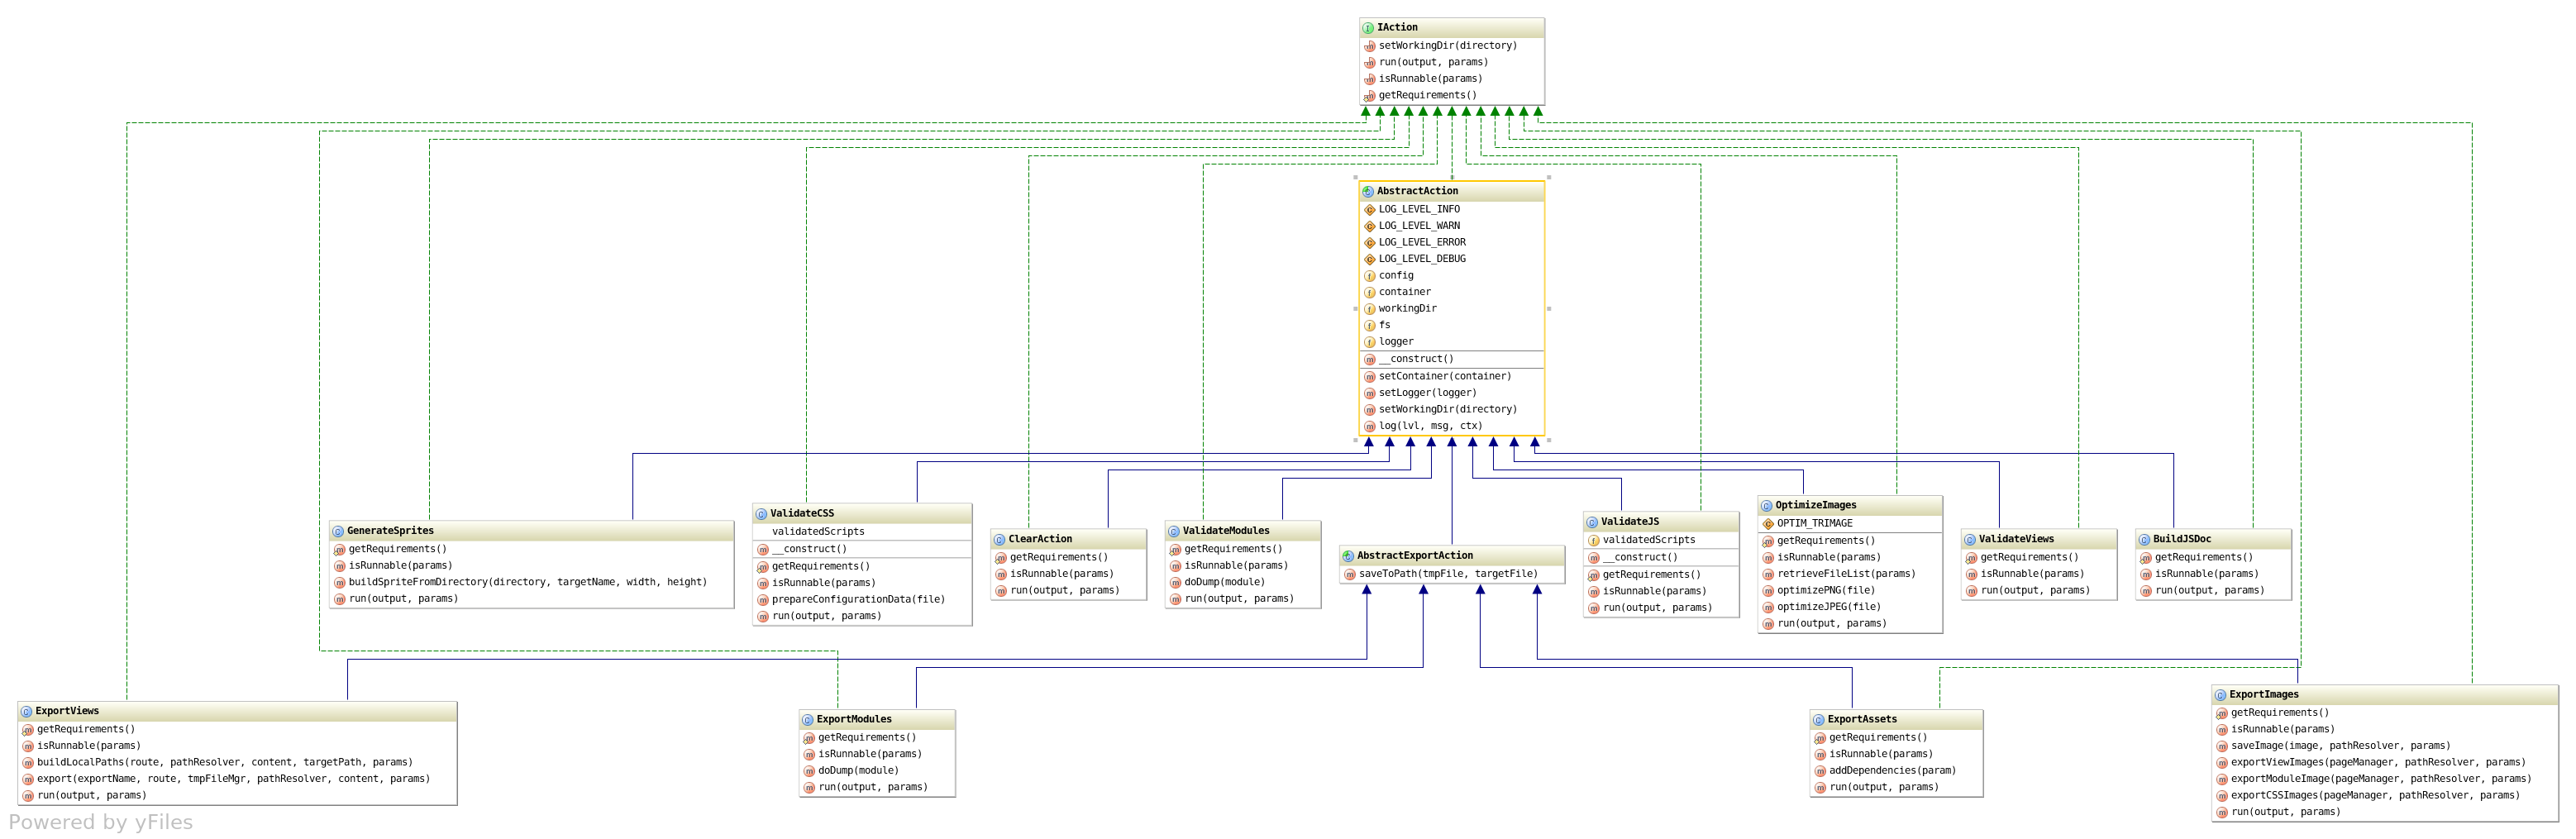
\includegraphics[width=21cm]{diagram.png}
\end{landscape}

\subsection{PHPDocumentation}


\end{document}